
\chapter{Architecture}

\section{Vaadin Architecture Overview}
\label{sec:vaadin-architecture}


Our system is a \textbf{\vaadin based java web application}. It is
composed by a server-side frontend, a Java EE 6 backend running on
glassfish, and a data subsystem currently using MySQL.
%
Let's start overviewing the generic vaadin architecture, as depicted
in (Figure~\ref{fig:vaadin-architecture}).
%
\begin{figure}[htpb]
  \centering
  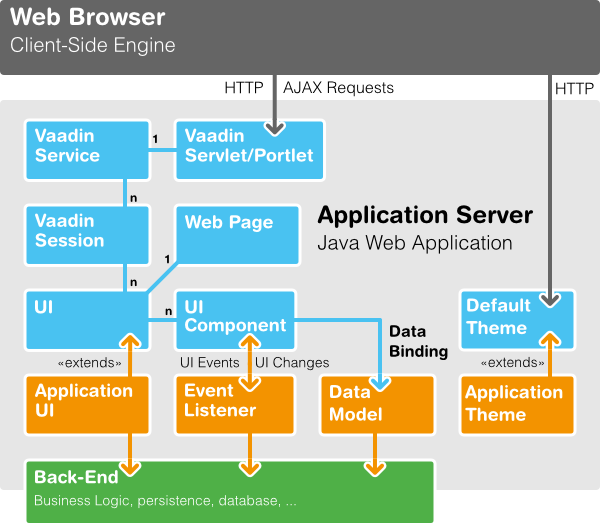
\includegraphics[scale=0.5]{figures/application-architecture-lo.png}
  \caption{Vaadin Java Web Application Architecture}
  \label{fig:vaadin-architecture}
\end{figure}
%
\begin{enumerate}
\item Web Browser. Contains the client-side engine of the web
  application. User interaction will result in request been sent to
  the server.

\item Vaadin Servlet/Portlet. Every request is intercepted and handled
  by a servlet. Servlets are server-side components that handle
  incoming requests, redirecting them as expected. They are associated
  with a Vaadin Service.

\item Vaadin Service manages the application sessions, keeping request
  integrity among distinct sessions.

\item Vaadin Session, manages user session and related data. During
  its lifetime a session may interact with one or more UIs.

\item UI. This is the top-level abstract class defining an application
  frontend. It intermediates all interaction between the user, the
  brwoser and the communication with the back-end. Our architecture
  cuts in providing an application user interface that extends the
  functionality of UI.

\item Application UI, a generic term referring a concrete
  implementation of UI. In our case that is the
  \code{LifetimeUI}. \code{LifetimeUI} is responsible to create the
  views to the user, depending on the url passed to the browser.

\item UI Components, we generally call them \emph{Views}, are the
  visible part of the application. They present the user with the set
  of possible actions; according to this architecture they must also
  register listeners to listen for user initiated events. In
  \lifetime, the top abstract class defining a view is the class
  \code{LifetimeView}, responsible to show the application visible
  part as well as to listen to all events inside it's internal
  structure.

\item Listeners react to diverse user actions (internally converted as
  events). Important subsystems depend on listener logic to make the
  application progreed. \textbf{Progress} is an important system
  property, that must be specified, enforced and tested. We use
  \emph{session types} to specify navigational progress, ensuring that
  use cases start, run and terminate as expected.

\item Themes allow modular definition of appearace properties of the
  web application, using \code{sass} or \code{less} as css-based
  languages.

\item Back-End. Services offered to clients are in the business logic
  subsystem, and persistent storage for application data in the
  persistence subsystem. Together with series of restfull web-services
  and message-queues they compose the application back-end.

\item Data Model, implements a variation of the \emph{MVC design
    pattern}, the \emph{MVP design pattern}, alliaviating the burn of
  having the controller to update both the model and the views. By
  associating a data model, this pattern allow us to have the user
  data automatically synchronized to a server-side persistent data
  transparently, using a process known as \emph{data binding}.

\end{enumerate}
%

%
The purpose of this chapter is to determine how to extend the \vaadin
architectural pieces to produce a specific architecture for
\lifetime. In the next sections we will specify \lifetime's specific
impementation of the \vaadin architecture.
%


\section{Lifetime Frontend Subsystem}
\label{sec:frontend}
The front-end subsystem is composed by composed by two main blocks:
\code{LifetimeUI} hierarchy and \code{LifetimeView}
hierarchy. According to the architecture listeners and data models
belong to \code{LifetimeView} architectural block, and together they
provide the means users access application use cases.
%
The front-end subsystem defines the \code{LifetimeUI} class hierarchy,
the \code{LifetimeView} class hierarchy, and a factory to create these
views. This configuration is presented in \ref{fig:lifetime-frontend}.
%
\begin{figure}[htpb]
  \centering
  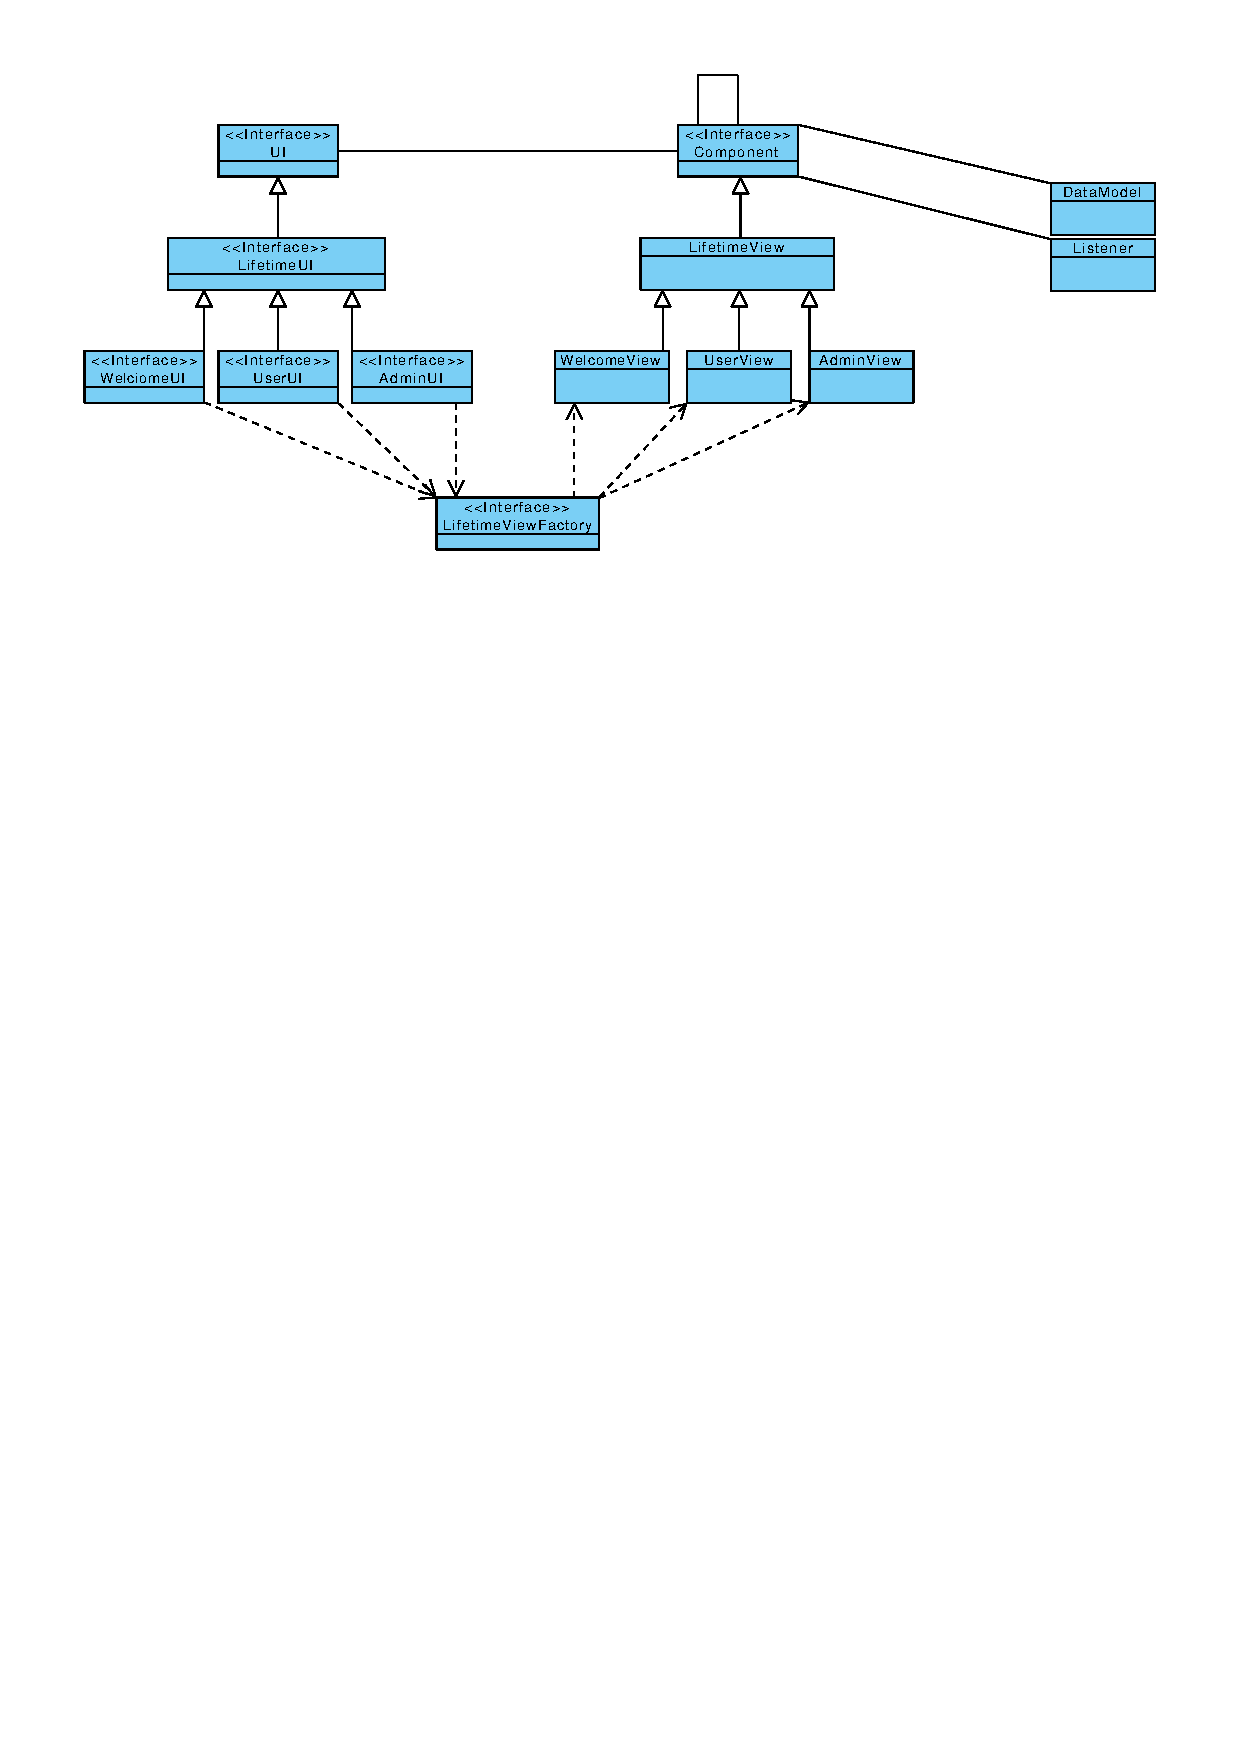
\includegraphics[scale=0.75]{figures/lifetime-frontend.pdf}
  \caption{Lifetime Frontend}
  \label{fig:lifetime-frontend}
\end{figure}
%


%
\subsection{LifetimeUI}
\label{sec:lifetimeui}

\code{LifetimeUI} extends from vaadin \code{UI} class. Our system
features multiple user roles, depending on the service subscription
level. At least the following roles must exist in \lifetime:
\begin{itemize}
\item Guest, to access unsecure parts of the app, like the welcome
  page, accessible to everyone
\item User, to access user area
\item Admin, for super-user app access
\end{itemize}
%
The \code{LifetimeUI} and subclass are reponsible to enforce among
others the security requiriements of the program. For each role we
provide a subclass of \code{LifetimeUI}, to correctly handle client
requests:
%
\begin{itemize}
\item \code{WelcomeUI}, handles requests to the unsecure part of our
  app
\item \code{UserUI} handles requests to the user area,
\item \code{AdminUI} handles requests to the admin area,
\end{itemize}
%
The \code{LifetimeUI} (and the subclasses) are reponsible for
initiating the correct \code{LifetimeView}, according to the user role
interacting with the system.

\subsection{LifetimeView}
\label{sec:lifetimeview}
\code{LifetimeView} extends from \vaadin \code{Component} class, and
they are initiated during the \code{init} method of the a
corresponding \code{LifetimeUI} subclass. They are created by a
role-dependent view factory.
%
In our application we consider the following views:
\begin{itemize}
\item \code{WelcomeView}, to access unsecure services like registering
  a new user account or reading the app contact page
\item \code{UserView}, to access user services, like \vitae
\item \code{AdminView}, to help administrating the application
\end{itemize}

\section{Lifetime Backend Subsystem}
\label{sec:backend}

\section{Lifetime Storage Subsystem}
\label{sec:storage}


%%% Local Variables:
%%% mode: latex
%%% TeX-master: "main"
%%% End:
